% Fun With SQL
\documentclass{beamer}
\usefonttheme{serif}
\usefonttheme{structuresmallcapsserif}
\usepackage{fancyvrb}

\begin{document}
\title{What's a Data Warehouse?}

\begin{frame}{Data Warehouse Differences}
    Data warehouse (OLAP) databases differ from transaction processing (OLTP)
    databases in (at least) the following ways:
    \begin{itemize}
        \item Purpose 
        \item Data sources 
        \item Style of queries, and usage patterns 
        \item Data organization 
    \end{itemize}
\end{frame}

\begin{frame}{Purpose}
    Data warehouses exist to allow users to query through piles and piles of
    old data.

    Data structures and levels of detail change over time; the data warehouse
    has to standardize all this.
\end{frame}

\begin{frame}{Data Sources}
    Data in a warehouse can come from all over: various databases, text files,
    web services, other stuff. The warehouse has to know how to talk to all
    these data sources.

    The ETL (Extract, Transform, Load) does the following:
    \begin{itemize}
        \item Extracts new / modified / whatever from the data sources
        \item Transforms the data into the structure the warehouse expects
        \item Loads / merges the new data into the database
    \end{itemize}

    Sometimes SYNONYMs are useful...
\end{frame}

\begin{frame}{Query style}
    Queries are:
    \begin{itemize}
        \item ...expected to take a while
        \item ...usually read-only (transactions don't matter)
        \item ...generally aggregate data
        \item ...sometimes return tons of data
    \end{itemize}
\end{frame}

\begin{frame}{Data structure}
    OLTP databases are modeled on "entities". OLAP databases are
    "dimensionally modeled". Essentially this means the table structure
    reflects various business processes (sales, hiring, orders, web site
    visits, admissions, etc.)
\end{frame}

\begin{frame}{Grain}
    To build a set of tables, start with the "grain", or lowest level of
    detail this set of tables will contain. Define this very clearly.
\end{frame}

\begin{frame}{Star schema}
    One table contains all the facts specific to one instance of your grain
    and no other (sale price, number of items in cart). This is the fact
    table. Data items that are identical across a set of instances of the
    grain are "dimensions" (customer, retail store, product SKU), stored in
    dimension tables. The fact table contains foreign keys to the dimensions,
    making a star-like design.
\end{frame}

\begin{frame}{Design considerations}
    \begin{itemize}
        \item Avoid null values and outer joins
        \item Use synthetic primary keys
        \item Reuse dimension tables in ohter stars, with other fact tables
    \end{itemize}
\end{frame}

% Data organization: ERD == Entity-Relationship Diagram. Common in typical
% database world because databases are modeled on "entities". So you have an
% orders table, an order lines table, a customer table, a user table, etc. DWs
% are dimensionally modeled. This means in practice that a database is modeled
% following various business processes. Hiring, sales, orders (multiple levels
% of orders here), transactions (banks might want a process to show daily
% traffic, monthly gain/loss, and a few other things). This process defines
% what's called the "grain", or the granularity of the data involved; choosing
% and defining the grain is the most important first step. They use a "star"
% schema, which means one central table (called the fact table) and several
% smaller "dimension" tables joined directly to it, making a star (sometimes the
% dimension tables are themselves kinda star-like, making it a snowflake schema,
% but these are best avoided). Facts include all the data specific to an
% instance of your grain (a sale, a transaction, etc.) that isn't going to show
% up identically in other instances (sale price, deposit amount, length of
% stay). Those things that do appear in multiple instances of the grain are
% dimensions (retail location, customer, product SKU, etc.). Dimension tables
% include all necessary attributes of a particular dimension (name, address,
% age, for instance). The fact table includes all the facts, plus foreign keys
% to the relevant dimensions. All tables generally include synthetic primary
% keys. NULL values should be avoided; so should OUTER joins. The ETL process
% gets complex when you start to think about looking up and merging in
% pre-existing dimensions, or dealing with changing dimensions.

\begin{frame}{OLAP}
    \begin{center}
        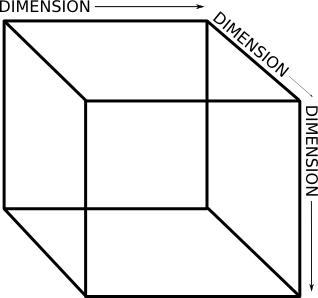
\includegraphics[width=0.8\textwidth]{cube.png}
    \end{center}
\end{frame}

\begin{frame}{OLAP}
    \begin{center}
        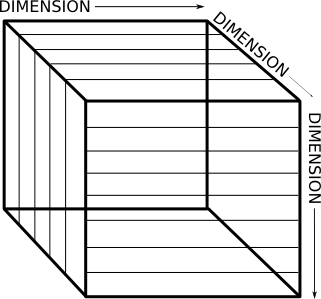
\includegraphics[width=0.8\textwidth]{cube-divided.png}
    \end{center}
\end{frame}

\begin{frame}{OLAP}
    \begin{center}
        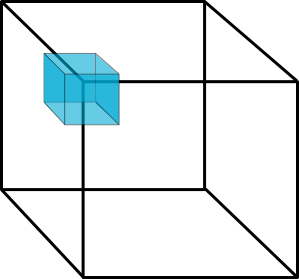
\includegraphics[width=0.8\textwidth]{cube-selection.png}
    \end{center}
\end{frame}

\begin{frame}{OLAP}
    \begin{center}
        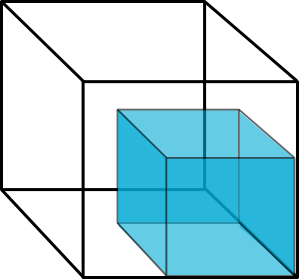
\includegraphics[width=0.8\textwidth]{cube-bigselection.png}
    \end{center}
\end{frame}

\begin{frame}{OLAP}
    \begin{center}
        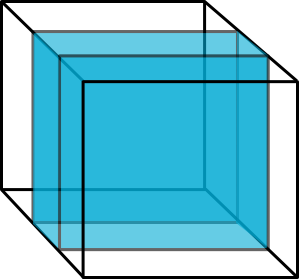
\includegraphics[width=0.8\textwidth]{cube-slice.png}
    \end{center}
\end{frame}


\begin{frame}{OLAP}
    \begin{center}
        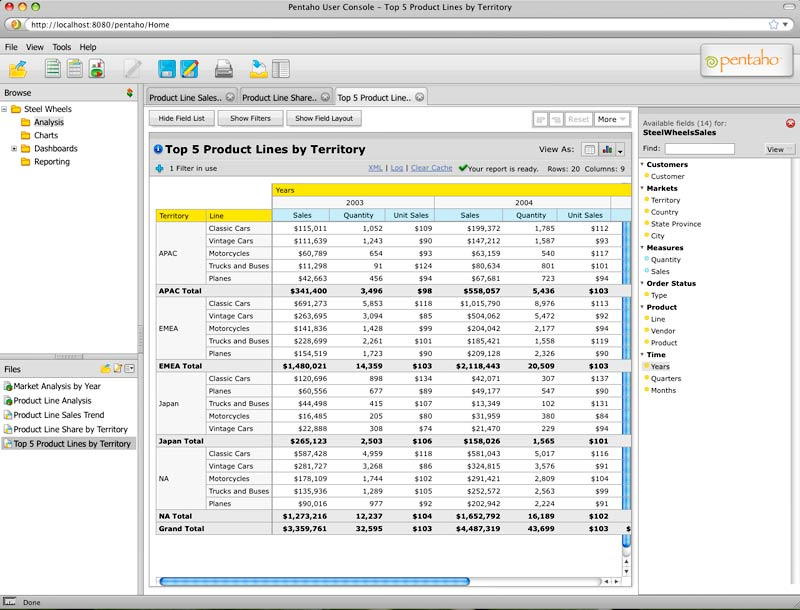
\includegraphics[width=0.8\textwidth]{analyzer.png}
    \end{center}
\end{frame}
%Tools:
%* Various reporting tools handle the relatively simple relationships of these
%tables well, for building reports using nice graphical builders.
%
%* MDX treats these tables as a "cube" with as many dimensions as there are
%dimensions in the database. Each dimensino has various possible values,
%dividing that dimension into segments. MDX tools allow users to select
%different segments of whatever dimensions they're interested in, and look at
%aggregate "measures" (facts) from the set of all data in those segments.
%http://www.titegypt.com/images/pentaho/analyzer_top5.jpg

\end{document}
